%%%%%%%%%%%%%%%%%%%%%%%%%%%%%%%%%%%%%%%%%
% University/School Laboratory Report
% LaTeX Template
% Version 3.1 (25/3/14)
%
% This template has been downloaded from:
% http://www.LaTeXTemplates.com
%
% Original author:
% Linux and Unix Users Group at Virginia Tech Wiki 
% (https://vtluug.org/wiki/Example_LaTeX_chem_lab_report)
%
% License:
% CC BY-NC-SA 3.0 (http://creativecommons.org/licenses/by-nc-sa/3.0/)
%
%%%%%%%%%%%%%%%%%%%%%%%%%%%%%%%%%%%%%%%%%

%----------------------------------------------------------------------------------------
%	PACKAGES AND DOCUMENT CONFIGURATIONS
%----------------------------------------------------------------------------------------

\documentclass{article}

\usepackage[version=3]{mhchem} % Package for chemical equation typesetting
\usepackage{natbib} % Required to change bibliography style to APA
\usepackage{gensymb}
\usepackage{textcomp}
\usepackage[utf8]{inputenc}
\usepackage{fullpage}		% margins
\usepackage{indentfirst}	% auto-indent
\usepackage[per-mode=fraction]{siunitx}
\usepackage{listings}
\usepackage{graphicx}
\usepackage{color}
\usepackage{amsmath}
\usepackage{mathtools}
\usepackage{enumitem}
\usepackage{float}
\usepackage{epstopdf}
\usepackage[margin=0.5in]{geometry}
\usepackage[format=plain,
labelfont={bf,it},
textfont={bf},
margin=2cm]{caption}

\setlength\parindent{0pt} % Removes all indentation from paragraphs

\renewcommand\thesection{\arabic{section}.}
\renewcommand\thesubsection{\alph{subsection})}

%\renewcommand{\labelenumi}{\alph{enumi}.} % Make numbering in the enumerate environment by letter rather than number (e.g. section 6)

% Commands and stuff
\newcommand\numberthis{\addtocounter{equation}{1}\tag{\theequation}}
% Code display stuff
\definecolor{backcolour}{rgb}{0.95,0.95,0.92}
\lstdefinestyle{mystyle}{
	backgroundcolor=\color{backcolour},   
}
\lstset{style=mystyle}


\title{{ECSE-426 Microprocessor Systems} \\[1in] {\bfseries {\small Group 12} \\ LAB 2 REPORT \\[5cm] }}
\author{Jaeho Lee \\ ID :260633759 \and Bobak Hamed-Baghi \\ ID: 260638423 \\}
\date{\today}


%----------------------------------------------------------------------------------------
%	DOCUMENT INFORMATION
%----------------------------------------------------------------------------------------
\begin{document}

\maketitle % Insert the title, author and date
\vfill

 \begin{abstract}
Micro-Controllers commonly have multiple different sensors to receive analogue data. Temperature sensor is one of the critical sensors which checks whether microchip is not overheating which can damage chip. This experiment is mainly focusing on receiving temperature of microchip using temperature sensor. Additionally, a LCD display was used to display the temperature data. The system was designed to display temperature in Celsius.  When an user interface (switch) receives signal, the temperature in Fahrenheit would display. A FIR filter was implemented to filter out noisy data read from the sensor. When the sensor sense high temperature, 40\, \celsius in the experiment, LED on the board are designed to alarm the condition.
 \end{abstract}
\newpage
%----------------------------------------------------------------------------------------
%	SECTION 2
%----------------------------------------------------------------------------------------

\section{Problem Statement}
The lab aims to achieve the following with the STM32F407SVG discovery development board:

\subsection{Temperature data acquisition}
The development board houses an ARM M4 microprocessor, which in turn houses a temperature sensor. This temperature sensor is internally wired to an analog to digital converter unit (ADC) which can be used to read the value of the sensor. In this lab we aim to read the value of the temperature sensor using the ADC, interpret the value into a meaningful measurement of temperature in both degrees Celsius and Fahrenheit scale, and implement direct memory access (DMA) to directly interface the ADC with device memory to save CPU cycles from being wasted. 

\subsection{Temperature display and alarm}
The STM32F407SVG board has many general purpose input and output (GPIO) pins which can be used to interface with external peripherals. In this lab we aim to interface the board with an external four digit seven segment display in order to display the temperature information in a human friendly manner. This involves configuring the required GPIO pins correctly and assembling the seven segment display circuit correctly. Furthermore, the lab requires that the on-board LEDs of the dev. board be lit up in a circular pattern following an overheat event, in which the CPU temperature is too high according to a threshold. This is done to alert the user immediately.

\section{Theory and Hypothesis}

\subsection{Temperature Calculation}
The temperature sensor output voltage varies linearly with temperature which can be read with the ADC peripheral. The sensor can measure temperature between \(-40\, \celsius ~ 125\, \celsius \). Below are the equations used for the calculations. Equation (1) was taken directly from the reference manual of the development board\cite{stm32ref}, and is used to calculate the temperature in degrees Celsius from the the analog voltage reading of the ADC, dubbed 'S'. Note that the division by 4096 is due to the fact that a 12-bit ADC mode was used, giving us 4096 voltage levels. Equation (2) is used to calculate the temperature reading from degrees Celsius to Fahrenheit for display when the button is pressed. 

\begin{align}
\text{temperature}(\, \celsius) &= 400\times S \times\frac{3.6}{4096} + 25 \\
\text{temperature}(^{\circ}F) &= 1.8*\text{temperature}(\, \celsius) + 32
\end{align}
\subsection{ADC initialization}
In order to initialize the ADC, there are several commands were made. ADC is using 12 bit to data display resolution. It aligns all the data into right, and disable conversion in both scanning and continuous mode since these are not needed for the experiment. DMA is also disabled since direct memory access is not the main goal of this experiment. Only one ADC is used in this experiment which leads number of conversion to be 1. In order to overrun detection is automatically enable, ADC\_EOC\_SINGLE\_CONV was use for EOCSelection.  
\subsection{GPIO pin initialization}
To initialize the GPIO, several commands were made. We defined short-cut of displaying numbers in LCD. All the pins implemented on board were called and clocks are enabled so we can used them to connect board to LCD display. GPIOA, GPIOE, and GPIOD were called where they represent different types. GPIOD represents which LCD light illuminates to show number. Each pin represents which digit is enabling. GPIOE represents which line on LCD illuminates. The combination of GPIOE pins shows which number is displaying. GPIOA represents external interrupts with falling edge sensitivity. In this case, switch which would switch Celsius to Fahrenheit is the external interrupt.
\section{Implementation}
A Detail flowchart of system operation is provided in appendix.
\subsection{Data Display}
For displaying data, four digit 7-segment display was used. Individual segment can be controlled by using general purpose input output (GPIO) pins implemented on the Micro-controller unit. Figure 1 shows how 7-segment LCD display is consisted.

\begin{figure}[!htb]
\begin{center}
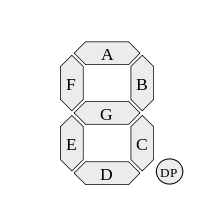
\includegraphics[width=0.40\textwidth]{7segment} % Include the image placeholder.png
\caption{7-segment LED display}
\end{center}
\end{figure}

To display each digit from 0 to 9, each number was defined separately. List of bit sequence to display number is follow in table.\\
\begin{center}
\begin{tabular}{lclclclclclc|cl}
a&b&c&d&e&f&g&display\\
\hline
1&1&1&1&1&1&0&0\\
0&1&1&0&0&0&0&1\\
1&1&0&1&1&0&1&2\\
1&1&1&1&0&0&1&3\\
0&1&1&0&0&1&1&4\\
1&0&1&1&0&1&1&5\\
0&0&1&1&1&1&1&6\\
1&1&1&0&0&0&0&7\\
1&1&1&1&1&1&1&8\\
1&1&1&0&0&1&1&9
\end{tabular}
\end{center}

\subsection{Data Filtering}
After receiving data and display in LCD, we could observe due to noisy data and frequency of sensor acquisition is extremely fast for human observation (100 Hz), a FIR filter was used to filter out the unnecessary noise and smooth output. Figure 2 briefly explain how FIR filter operates. in this lab, an average filter was used to smooth display output. 50 kernel inputs were used which delays the first output and reflect of extreme temperature change by 0.5 second however smooths the graph.

\begin{figure}[!htb]
\begin{center}
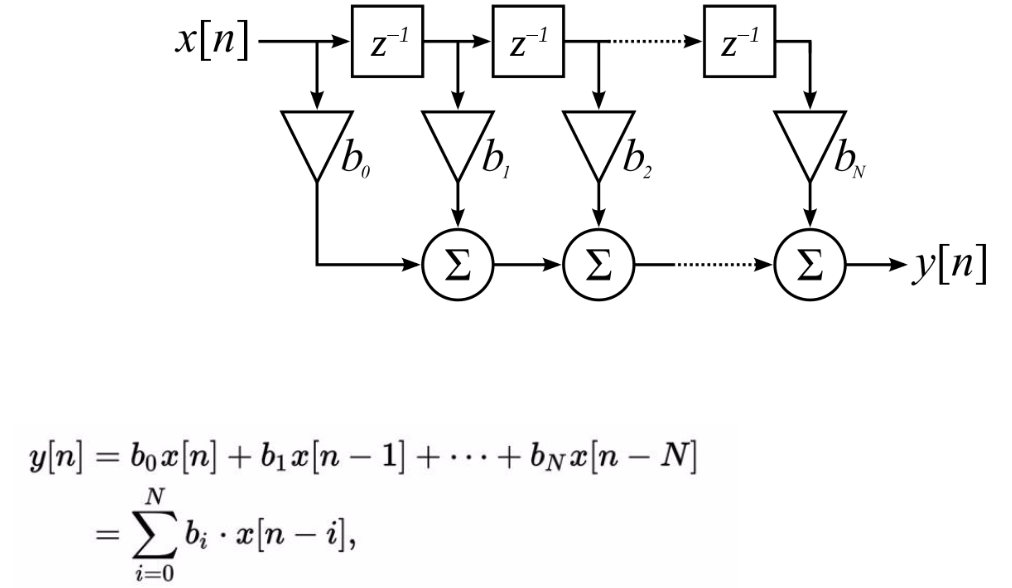
\includegraphics[width=0.70\textwidth]{FIR.png} % Include the image placeholder.png
\caption{FIR filter}
\end{center}
\end{figure}

\subsection{Timing}
In order to perform the system properly, a source of periodic timing is required. SysTick timer is implemented in the MCU and was used to control frequency of operation. In this experiment, SysTick decrements the frequency down to 100Hz. 

\subsection{Alarm}
The system was designed to alarm the user if the microchip is overheating which may cause damage. In this system, 4 LEDs implemented on board are design to illuminate. In order to emphasize the warning, each LED illuminates in clockwise order. In order to implement this, LED dance function was designed and in every 250ms, each LED illuminates in clockwise order.

\section{Testing \& Observations}
In the first prototype, we modified System clock configuration-given code-in order to clock down system from 1 kHz into 100 Hz. However during the first test with LCD light, we observed data does not display properly since we have clocked down, it results data collision. Therefore we made an extra if statement in main while loop which counts every cycle and every 10 cycle, which gives 100 Hz speed, LCD display operates to show the current data. We also observed that the data is very unstable, human eye cannot follow the number properly [1]. We initially implemented FIR filter which we used in previous lab. This filter has 5 kernel inputs shapes Gaussian distribution. This filter could not smooth data enough, we decided to increase number of kernel inputs. Increasing kernel inputs can delay data appearance if sensor data changes drastically. However consider the clock speed, we concluded that delay of 250ms is worthy if we can smooth data enough. We used 50 kernel inputs which smoothed data properly. When external user interface-a switch implemented on the board-receives signal from user, the data changes to Fahrenheit immediately and display Fahrenheit instead of Celsius. Whenever the temperature of microchip is higher than the threshold temperature, 40 Celsius, LED light implemented on the board illuminates to notice the user.

\section{Conclusion}
The system successfully initialized ADC and GPIO pins. It received sensor data from temperature sensor and calculate into regularly used temperature units (Celsius and Fahrenheit). Whenever user interface receives signal from user, it successfully switches display between Celsius and Fahrenheit. And it could warn the user if the temperature of microchip is above the threshold temperature.

\begin{thebibliography}{9}
\bibitem{Response Time Measurement} 
Simon Baker. 
\textit{Response Time Measurement}. 
TFT Central, Reading, UK, 2013.
 
\bibitem{STMicroelectronics} 
{RM0090 Reference manual STM32F405/415, STM32F407/417, STM32F427/437 and STM32F429/439 advanced\\ ARM{\textregistered}-based 32-bit MCUs},
\\\texttt{http://www.st.com/content/ccc/resource/technical/document/reference{\_}manual/3d/6d/5a/66/b4/99/40/d4\\/DM00031020.pdf/files/DM00031020.pdf/jcr:content/translations/en.DM00031020.pdf}
\end{thebibliography}

\bibliographystyle{unsrt}
\bibliography{sample}

\newpage
\section{Appendix}
\begin{figure}[!htb]
\begin{center}
\includegraphics[width=0.8\textwidth]{flowchart.png} % Include the image placeholder.png
\caption{Flowchart detailing the operation of the system.}
\label{fig:fc}
\end{center}
\end{figure}


\end{document}